\documentclass[10pt,a4paper,twoside]{book}


\usepackage[utf8]{inputenc}
\usepackage[english]{babel}
\usepackage[english]{isodate}
\usepackage[parfill]{parskip}

\usepackage{graphicx} 
\usepackage{hyperref}

\newcommand{\progname}{dclamp}

\title{\textbf{\progname} \\ command-line electrophysiology \\ User manual}
\author{Daniele Linaro \\ Jo\~ao Couto \\ Michele Giugliano}
\date{}
\hypersetup{
 pdftitle = {\progname, command-line electrophysiology},
 pdfkeywords = {electrophysiology,dynamic clamp,real-time},
 pdfauthor = {(Daniele Linaro, Joao Couto and Michele Giugliano)}
}

\begin{document}

\maketitle
\thispagestyle{empty}

\pagenumbering{roman}
\tableofcontents
\newpage
\pagenumbering{arabic}
\chapter{Getting started}
\label{chapter:start}
\paragraph{}
This chapter will help you understanding some basic concepts related to \progname. It starts by giving a notion of the basic commands using an artificial neuron and continues to interfacing with live cells. While it does not intend to be a detailed tutorial on either matlab nor python, some indications on how to use these software packages will be provided.

\section{Requirements}
\paragraph{}
In order to get started you need only to boot your computer into the live DVD/USB (available at \url{http://www.tnb.ua.ac.be/LCGliveCD.iso}). Instructions on setting up live USB medium are available in section \ref{note:liveUSB}.
Although all experiments can be performed from the live medium, for production environments, it is better to have a dedicated installation of LCG. We provide debian kernel packages with  the PREEMPT\_RT kernel patch for simple installation in Debian like systems. Additional notes on the installation can be found in section \ref{chap:installation}).

\paragraph{}If you are using a system that someone else installed you can check wether \progname is installed  by typing  \texttt{which \progname} in a terminal window; if the result is blank, the program has not been installed and you should either use the live DVD or install it yourself. 

\paragraph{}
We assume that can open a terminal window in the Linux distribution that you are using and will slowly introduce some concepts from there however this does not intend to be a tutorial on using Linux. 
Check the webpage of your linux distribution (e.g. \href{http://www.debian.org}{Debian}; \href{http://www.ubuntu.com}{Canonical Ubuntu}; \href{http://www.fedoraproject.org}{Fedora}) or the \href{http://www.linux.org/tutorial}{linux.org} tutorials for help on getting started with Linux. Additionally, the \emph{Advanced Bash-Scripting guide} from \href{http://www.tldp.org}{The Linux Documentation Project} is a great reference for how to use a UNIX terminal efficiently.

\paragraph{}
Some MATLAB and Python code will be used to demonstrate the basic loading of data. Knowledge of these languages can be beneficial.
Before getting started using \texttt{\progname} you may want to take a look at Appendix \ref{appendix:matlabReference} for a short Matlab introduction and Appendix \ref{appendix:unixReference} for some notes on UNIX basic commands.

\section{Introduction - What is \progname?}

\paragraph{}
In short \textbf{\progname} is the name of a UNIX program that interfaces with \texttt{lib\progname}\  - a C++ library that can be used to conduct electrophysiological experiments using simple stimulation protocols but also highly complex paradigms such as hybrid networks interfaces and/or dynamic clamp. 

% If you are an experienced programmer and you want to interface with lib\progname\, consult the Doxygen documentation and the source code in \href{https://github.com/danielelinaro/dynclamp}{GitHub}.



%%%%%%%%%%%%%%%%%%%%%%%%%%%%%%%%%%%%%%%%%%%
% The following is commented out
\iffalse

\section{Configuration files}
\paragraph{}
A configuration file is a Extensible Markup Language \emph{xml} file and can be opened in a standard text editor (\texttt{gedit <filename>} or \texttt{vi <filename>}). Examples can be found in the examples folder of the \progname\ source code or in the webpage of \href{http://www.tnb.ua.ac.be}{\progname}.

\paragraph{}
The basic building blocks of \progname\ are called entities. An experiment consists of the interaction of several entities. We communicate with \progname\ by describing how the entities are connected to each other in a configuration file. Check section \ref{chap:entities} for a description of the built in entities.

Lets examine one of these files closely:

\renewcommand{\lstlistingname}{Example}
\begin{lstlisting}[caption={A simple example of a configuration file with a simulated integrate and fire neuron.},label={gettingStarted:example0},language=XML,morekeywords={dynamic clamp,entities,entity,name,id,C,tau,tarp,Er,E0,Vth,Iext,parameters,connections,simulation,tend,rate}]
<dynamicclamp>
  <entities>
    	<entity>
      		<name>LIFNeuron</name>
      		<id>1</id>
      		<parameters>
			<C>0.08</C>
			<tau>0.0075</tau>
			<tarp>0.0014</tarp>
			<Er>-65.2</Er>
			<E0>-70</E0>
			<Vth>-50</Vth>
			<Iext>220</Iext>
      		</parameters>
      		<connections></connections>
    	</entity>
  </entities>
  <simulation>
  	<tend>5</tend>
   	<rate>20000</rate>
  </simulation>
</dynamicclamp>

\end{lstlisting}
 
This file is composed layers. The most general is the \texttt{<dynamicclamp>} layer; this basically tells the program that this is a configuration file. Inside this layer there are two other:
\begin{itemize}
\item
\emph{ \texttt{<entities>}}  - where the entities are listed and connected to each other. Generally each \emph{ \texttt{<entity>}} has a 
	\begin{itemize}
	\item \emph{ \texttt{<name>}} - the global descriptor of the entitiy. 
	\item \emph{ \texttt{<id>}} - the global identification number of an entity. This is used to connect entities and the ids have to be unique.
	\item \emph{ \texttt{<parameters>}} - the parameters of the entity. These vary between each entity. You can use the manual section \ref{chap:entities}.
	\item \emph{ \texttt{<connections>}} - the global \texttt{id}s to which this entity is connected.
	\end{itemize}
\item
\emph{ \texttt{<simulation>}} - where the general parameters are defined e.g. the sampling rate (\texttt{rate}) and the duration (\texttt{tend}).
\end{itemize}

\paragraph{}
Now lets create a file called \texttt{example.xml}. Open a terminal and copy the following lines one by one:

\begin{lstlisting}[escapeinside=\{\}]
mkdir ~/examples  # this creates a directory called under your home folder (that's what the tilt is for)
cd ~/examples # goes inside this directory
gedit example1.xml # creates and opens a file called example.xml in the current folder using gnome text editor.
\end{lstlisting}

Note that if you do have a system without \texttt{gnome} like Mac OS the command \texttt{gedit} will not work; any text editor can be used. Now copy the example (\ref{gettingStarted:example0}) above to this file. If you use copy and paste make sure that there are \textbf{no extra spaces}, this will depend on the your choice of editor. Save and close it. You can now run the example by doing: \texttt{\progname\ -c example.xml}

The \texttt{-c} option stands for \textbf{configuration file} can be used to tell \progname\ that we are going to pass a configuration file as an argument.

\paragraph{} You have just ran a simulation of an integrate and fire neuron's membrane potential for 5 seconds. This was a very basic example, so the data was not recorded. In the next section you will see how you can record the data.
\fi
% END OF COMMENT OUT
%%%%%%%%%%%%%%%%%%%%%%%%%%%%%%%%%%%%%%%%%%%
\section{First steps in Command Line Electrophysiology}
\paragraph{}
The most important concepts of related to \progname can be understood by using a computational model of a neuron. Some single compartiment models are integrated in \progname; in this chapter we will a Linear Integrate and Fire model (for an introduction see: \cite{Koch:1989}). The initial part of this guide does not require a realtime kernel nor a data acquisiton board.
We will illustrate some basic concepts of data analysis of intracellular data using Python and Octave/Matlab. This should allow a user that is not familiar with Python nor \matlab\ to understand the basics and provide building blocks for more complete analysis. Please note that this does not intend to be a full fletched tutorial, of data analysis nor an introduction to computer programming. 

\paragraph{}A good reference for getting started with \matlab is \cite{wallisch2011} or the resources at \href{http://www.mathworks.com}{The Mathworks} website for Matlab; for Python we suggest the \href{https://scipy-lectures.github.io/}{Scipy lecture notes}. We will also try to highlight some basic UNIX commands to handle file operations  and suggest ways to structure and organize your experiments.

\subsection{Creating an experiment folder}
\progname does not require a particular folder structure to be used, i.e. when you run a command the recording will be executed in that very same directory. However it is very beneficial to use  a consistent folder structure. You can use \texttt{\progname create\_experiment\_folder} for that:

\begin{lstlisting}[numbers=none,language=bash]
lcg-create-experiment-folder -p YYYYMMDD_tutorial_[001] -s LIFsteps,steps 
\end{lstlisting}

Note that \texttt{lcg-create-experiment-folder} can do more than creating a folders i.e. it can add information files with details from the experiment, you can the read more about it in section \ref{lcg:create_experiment_folder}.

After running the above command you will see the name of the folder that was just created. Go into this folder using the \unix command \texttt{cd <foldername>}.
By using the command \texttt{ls} you can list the directories under this directory i.e. LIFsteps and steps.  \texttt{lcg-create-experiment-folder} also created a folder \texttt{01} inside each of these with the intention of storing different sets of trials with the same protocol.  In this way the first time the protocol was run would be stored in the \texttt{01} directory, the second in \texttt{02} and so on.

\subsection{Recording from a simulated neuron}

To get started lets compute the frequency-current (FI) curve of simulated Linear Integrate and Fire neuron. For this we will use the \texttt{lcg-steps} protocol with the \texttt{--model} option. 
Run the following commands in the terminal window (what follows \# is a comment).

\begin{lstlisting}[numbers=none,language=bash]
# Go into the stepsLIF/01 directory
cd LIFsteps/01
# Run the protocol
lcg-steps -a -200,800,50  -d 1 --model --no-shuffle -n 1
# Plot the results
lcg-plot -f all
\end{lstlisting}
One of the most important things that you should know is that each protocol as computed like this has multiple switches or options and that these usually have default parameters. Make sure that the default parameters fit your purpose otherwise use switches to set them. All protocols have a \texttt{--help} switch that displays the supported options and default parameters.

In the above example you used \progname to inject current steps from $-200$ to $800\pico\ampere$  with $50\pico\ampere$ increases and $1 \second$ duration into a simulated neuron. The \texttt{--no-shuffle} option makes that the steps amplitudes are not shuffled before applied.

\subsection{Loading files and analyzing data}
\paragraph{}Analyzing data is probably the most important step of an experiment. While this manual does not intent to go into details on the data analysis we will show examples of simple scripts to visualize and analyze data for this simple case.
\paragraph{} Before proceeding you should understand the basic structure of the data files recorded by \progname when using \hdf files. For a detailed explanation read chapter \ref{chap:datafiles}. Each file contains at least 2 groups \emph{Entities} and \emph{Info}. The \emph{Entities} group contains each element (entity; see \ref{chap:entities}) of the recording, in this case the recorded voltage trace and the injected current step. It should be noted that each entity can also contain \textbf{metadata} representing its parameters e.g. the stimuli parameters for the \emph{Waveform} entity. The \emph{Info} group contains parameters of the experiment such as the \emph{time step (dt)} used and the \emph{duration (tend)} of the recording.

\subsubsection{Python example}
The scientific community often uses Python to analyze data and produce publication ready figures. We will show you how to produce a simple figure from the recorded traces using the \texttt{ipython notebook} which is a neat way to interact with the Python interpreter. In its essence it lets you write and annotate the data analysis script from a standard Internet browser. For details on how to use Python you should follow a tutorial on-line.

Start by launching the notebook and creating a new document. 

\begin{lstlisting}[numbers=none,language=bash]
 ipython notebook --pylab
\end{lstlisting}

This should open a browser window and let you create a new notebook in the current working directory.
You can now write Python code and execute it directly in the browser. Start by writing the following:
\renewcommand{\lstlistingname}{Example}
\begin{lstlisting}[caption={An example of a how to use Python to plot all entities in a \hdf file recorded with \progname.},label={python:plot_entities},language=Python,upquote=true]
from glob import glob   # To list files
import numpy as np      # To handle numerical arrays and some math 
import pylab as p       # To plot and visualize
import lcg              # To load experiment files and more
# List experiment files
files = glob('*.h5')
# Load and investigate last file
fname = files[-1]
ent,info = lcg.loadH5Trace(fname)
# Look at the names of the entities 
print [e['name'] for e in ent]
# Thus the first entity is the Neuron and second entity the Waveform

# Create a time vector 
#(This is done using size of the data and the sampling rate (1/dt))
time = np.arange(len(ent[0]['data']))*info['dt']
# Plot the data in 2 plots with shared x axis
fig, ax = p.subplots(len(entities),1, sharex=True)
for i,e in enumerate(ent): 
    # Plot the data
    ax[i].plot(time, e['data'])
    # Add labels with the information from each entity
    ax[i].set_xlabel('Time (s)')
    ystr = '{0} entity ({1})'.format(e['name'],e['units'])
    ax[i].set_ylabel(ystr)
# Set the filename as title
ax[0].set_title('Data from file {0}'.format(fname))
\end{lstlisting} 

The code in listing \ref{python:plot_entities} can be used to plot all entities in a file. We will now use the metadata to extract information about the stimulus. Of course this could also be extracted from the current waveforms but becomes much easier from the metadata (specially for more complicated protocols).

By analyzing the current trace plotted before, we know that our stimulus consists of 1 sec recording followed by 1 sec of stimulus and 1 sec of recording. This is translates into a  protocol description (metadata, see \ref{chap:stimgen}) with 3 lines. The protocol code (second column) is the same for all rows. And the stimulation amplitude is therefore in the second row (third column). 

\renewcommand{\lstlistingname}{Example}
\begin{lstlisting}[caption= {Python example of the code to compute the spike rate during the stimulus for a LIF neuron.} ,label={python:spk_rate},language=Python, upquote=true]

# Get the metadata
metadata = ent[1]['metadata']
V = ent[0]['data']
# Cumulative sum of the first column is the duration 
prot_time = np.cumsum(metadata[:,0])
# The third column is the amplitude of the stimuli (for the DC protocols); we are interested in the amplitude of the second line since that is the one of the step of current.
stim_amp = metadata[1,2]
# Find the peaks that cross threshold
threshold = 0.0
# The following line is sufficient to detect the spike indexes by in the simulated neuron in real data another approach must be taken.
indexes = np.where(V >= threshold)[0]
spikes = time[indexes]

rate = len(spikes[(spikes > prot_time[0]) & (spikes <= prot_time[1])])/(prot_time[1]-prot_time[0])
print('The spike rate is {0} spikes per second for a current of {1}pA.'.format( rate, stim_amp))
\end{lstlisting}

The spike rate is then simply the number of spikes that happened during our current step divided by the duration

We can now iterate through all the files and compute the FI curve i.e. the spike rate versus the current.

\renewcommand{\lstlistingname}{Example}
\begin{lstlisting}[caption= {Python example of the code to compute the FI curve of a LIF neuron.} ,label={python:FI},language=Python]
def computeRateForLIF(time, V, metadata, threshold=0.0):
    # Function to compute the rate and return the stimulus amplitude
    # for a LIF neuron. See previous python code example.
    prot_time = np.cumsum(metadata[:,0])
    stim_amp = metadata[1,2]
    indexes = np.where(V >= threshold)[0]
    spikes = time[indexes]
    rate = len(spikes[(spikes > prot_time[0]) & (spikes <= prot_time[1])])/(prot_time[1]-prot_time[0])
    return rate, stim_amp

# List experiment files
files = glob('*.h5')
F = []
I = []
# Iterate through the files
for fname in files:
    ent,info = lcg.loadH5Trace(fname)
    V = ent[0]['data']
    metadata = ent[1]['metadata']
    time = np.arange(len(V))*info['dt']
    # Use our function
    tmp_rate,tmp_stim = computeRateForLIF(time,V,metadata)
    F.append(tmp_rate)
    I.append(tmp_stim)
# Make list an numpy.array to sort it so that plotting locks nicer
F = np.array(F)
F = F[np.argsort(I)]
I = np.sort(I)
# Plot and add axis labels
p.plot(I,F,'ko-', clip_on=False)
p.xlabel('Current (pA)')
p.ylabel('Rate (spikes per second)')
p.grid(True)
\end{lstlisting}

Example \ref{python:FI} illustrates how to iterate through multiple files using Python. We would recommend that users not familiar with Python and willing to use it for data analysis engage in 2 simple exercises before continuing:
\begin{itemize}
\item{} compute the voltage-current (VI) curve for the traces where the LIF neuron does not fire and deduce the input resistance from the VI curve.
\item{} make a more general function for spike detection that finds the local maxima  of putative spikes (and hence works also for real data). 
\end{itemize} 

\subsubsection{Matlab example}

We will now see how to use \textbf{\matlab} to read this file and extract the timing of the spikes. 
First open \matlab\ in a terminal window with the command: 
\begin{lstlisting} 
matlab -nodesktop 
\end{lstlisting}

You should see something like:
\begin{lstlisting}[numbers=none,language=xml]
		< M A T L A B (R) >
Copyright 1984-2012 The MathWorks, Inc.
	R2012b (8.0.0.783) 64-bit (maci64)
		August 22, 2012

To get started, type one of these: helpwin, helpdesk, or demo.
For product information, visit www.mathworks.com.
 
>> 
\end{lstlisting}

We will use \matlab\ without desktop in these examples if you prefer to use the desktop mode, you can launch \matlab\ with the command \inlineCode{matlab &}; all this assuming \matlab\ binaries have been added to path.
\matlab\ can be used to automate the analysis method in a highly efficient manner however in this section we will focus on the basic concepts. Rest assured: once you get a grip of \matlab\ and \matlab\ functions you will greatly reduce the amount of time that you require to analyze these sort of traces.

\paragraph{\matlab\ functions and the path}

You could load these file only using the built in functions of \matlab\ to read HDF5 files however this would be rather time consuming. The basic notions of \matlab\ that you need to get acquainted with before continuing the are the concept of \texttt{functions} and \texttt{path}.

The terminal that you have in front of you is interactive and the commands you type there will be ran as \matlab\ commands. Some of the power of \matlab\ lays in how simple it is to create functions. A function can be seen as a generic box that receives inputs and returns outputs. The computations processed to transform the inputs into the outputs are the core of the function. In \matlab functions are defined by naming a file with the name of the function and placing the code \inlineCode{function [out] = functionName(in)} in the first line of that file.

This said, \matlab\ functions are just files which are named the same as the function. \matlab\ does not search for functions in all directories of your disk (this is a very good thing!) and because of that you have to tell \matlab\ where to search for functions. In order to do so you can use the \texttt{add path} command. 

Every \matlab\ function/command has a documentation built in. You can access this by typing \inlineCode{help <name>}.

Now you need to add the functions that ship with \progname\ to the path (in case they are not already there). You can do this (for the current \matlab\ session) by doing:

\begin{lstlisting}[escapeinside=\{\}]
addpath([getenv('{\progname}_path'),'\matlab'])
\end{lstlisting}

Note that the above command will not work if you haven't defined the variable \texttt{\progname\_path} in your environment (\texttt{\$HOME/.bashrc} file) as the location of the source code of \progname. Although this command may seem complicated to the first time user of \matlab, the only thing it does is retrieving the environment variable '\texttt{\progname\_path}' and concatenating it with the \texttt{'\textbackslash matlab'} string. This because the we want to add the files that are in this folder to the \matlab\ path.

\paragraph{Loading and plotting the recorded traces}
Now that you added the function in the source path of \progname\ to the path of \matlab\ with the command:

\begin{lstlisting}[escapeinside=\{\}]
addpath([getenv('{\progname}_path'),'\matlab'])
\end{lstlisting}

The function \texttt{loadH5Trace} will be available for \matlab. Type \inlineCode{help loadH5Trace} to access the help of this function.
You can load and plot the data with the commands:

\begin{lstlisting}[language=matlab,morekeywords={loadH5Trace,ls},escapeinside=\{\}]
files = dir({\textquotesingle}*.h5{\textquotesingle});
[entities,info] = loadH5Trace(files(end).name)
entities(1).name
Vm = entities(1).data;
time = [0:length(Vm)-1]*info.dt;
plot(time,Vm,{\textquotesingle}k{\textquotesingle})
\end{lstlisting}

The first line uses \matlab 's command \texttt{dir} to list all directories. Then \texttt{loadH5Trace} loads the data into the variables \texttt{entities} and \texttt{info} -  it loads one structure per entity connected to the \nameref{entities:h5recorder} and thus we will think of it as a structure array (read about \matlab\ datatypes).

The third line in the above code is solely for illustration of how you can find out the name of an entity in the \texttt{entities} array. This can be particularly useful since it lets you find a particular entity based on it's type. Later we will see how to take advantage of this feature.
The fourth and fifth line we associate the variable Vm to the recorded membrane potential of the \nameref{entities:lifneuron} and create a time vector with the size of \texttt{Vm} and using the time step that is saved in the \texttt{info} structure.

The last line plots the time versus the voltage using the color black.

\paragraph{Detecting the peak of the spikes}

There are several ways of detecting the peaks of the spikes. We will focus on a relatively robust yet simple method of doing so by taking advantage of the \matlab\ function \texttt{findpeaks}.

\begin{lstlisting}[language=matlab,morekeywords={findpeaks,THRESHOLD,MINPEAKDISTANCE},escapeinside=\{\}]
% Define the refractory period of the peak detector (1ms); this can be useful when dealing with noisy signals.
refractory = 1.e-3/info.dt; 
% The following uses the function find peaks to find the spikes with threshold crossing at 0mV and a refractory period. 
[peaks, loc] = findpeaks(Vm,{\textquotesingle}THRESHOLD{\textquotesingle},0,{\textquotesingle}MINPEAKDISTANCE{\textquotesingle},refractory);
% The spikes are the locations of the peaks on the time vector
spks = time(loc);
% Plot time versus membrane potential
plot(time, Vm,{\textquotesingle}k{\textquotesingle})
hold on
% Plot the spike times and the peaks of the Action Potentials. The {\textquotesingle}hold on{\textquotesingle} command makes that the plots overlap.
plot(spks, peaks,{\textquotesingle}b.{\textquotesingle})
\end{lstlisting}

The above commands will get you to extract the peaks of the action potentials and the spike times and to plot them on the membrane voltage trace.
These commands should work also with very noisy signals, as long as the threshold and the refractory period are defined accordingly.

Now it would be useful to know the mean interspike interval. First we need to compute the interspike intervals, that can be easily done by using the \texttt{diff} command. 

\begin{lstlisting}[language=matlab,morekeywords={findpeaks,THRESHOLD,MINPEAKDISTANCE},escapeinside=\{\}]
% Compute te interspike intervals
isi = diff(spks);
% And the mean can be computed in a straight forward manner:
mean(isi)
% The reciprocal will give you the result in Hz
1./mean(isi)
\end{lstlisting}


\subsection{Interfacing with a Patch Clamp amplifier}

\progname is not bond to a particular amplifier or amplifier brand. While on one hand this adds versatility to the program, on the other it requires that the user is familiar with some of basic concepts of data acquisition and inner loops of the amplifier.

A recording system for patch clamp electrophysiology using \progname is composed of:
\begin{enumerate}
\item{Patch-clamp Amplifier}
\item{Data Acquisition Board} referred to as DAQ throughout this manual.
\item{Recording computer running \progname}
\end{enumerate}

Assuming that the DAQ board is supported by the \comedi drivers (or other drivers supported by \progname) then it is need that the recording computer understands what the values being read through the DAQ card mean in terms of the physical quantities being measured. This is accomplished in \progname by a set of environmental variables \footnote{If you do not know what a Bash environmental variable is, please refer to a Bash introduction course.}.

In essence we need to know:
\begin{enumerate}
\item{Where to measure from and what that measure means?}
\item{Where to stimulate to how to output something meaningful?}
\end{enumerate}
All this information is set up during installation (see section \ref{sec:configuration}) simply by editing a text file. 

\paragraph{}
\begin{figure}[h]
    \centering
    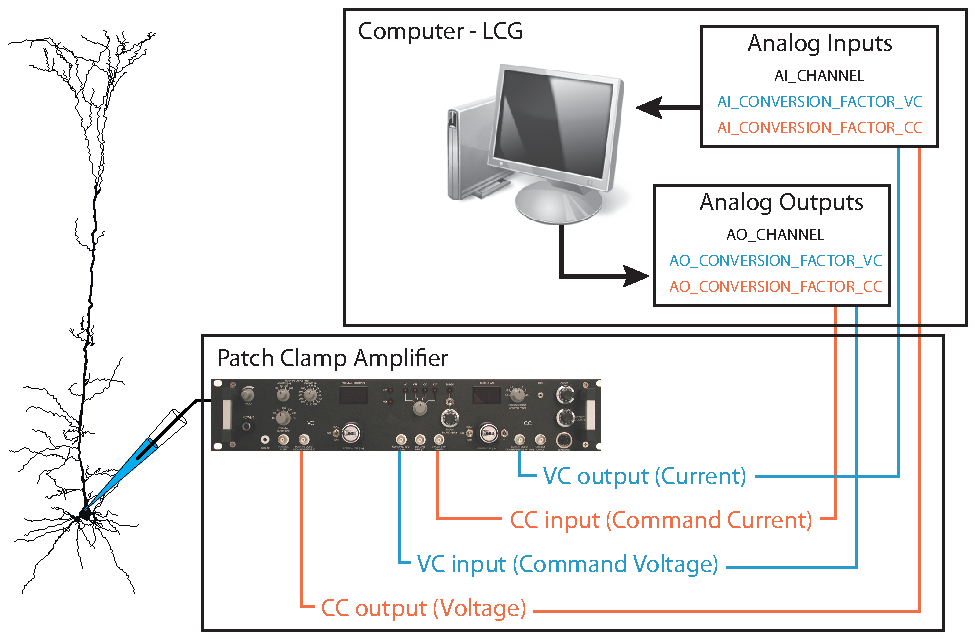
\includegraphics[width=0.8\textwidth]{figures/daq2amplifier}
    \caption{Correspondence between Digital Data Acquisition board and the patch clamp amplifier.}
    \label{fig:daq2amplifier}
\end{figure}

Figure \ref{fig:daq2amplifier} illustrates the most important connections and environmental variables that are involved in controlling the amplifier both in Current Clamp and in Voltage Clamp mode. Protocols ran in Current Clamp mode use the environmental variables with \textbf{CC} suffix while those ran in Voltage Clamp mode use the \textbf{VC} suffix which allows different gains, channels and units to be used with minimal interaction from the user side.
 
Most \progname protocols that support both voltage clamp and current clamp modes have a \textbf{--voltage-clamp} switch that instructs the program to use the proper conversion factors.

A small program called \textbf{lcg-find-conversion-factors} can help quickly discovering the conversion factors associated with the patch clamp amplifier.

\subsection{Your first recording}
Once you have configured the environmental variables as described in section \ref{sec:configuration}, \progname is ready to be used for patch clamp recordings.
 We can now attempt to characterize the VI and FI curves of a patched cell as for the simulated neuron. This can be accomplished simply by running the \textbf{lcg-steps} protocol. 

Set the amplifier to current clamp (CC) mode and enable the external command (if required by the patch clamp amplifier). You can now use Active Electrode Compensation to compensate pipette resistance errors so do not apply bridge compensation in the amplifier \footnote{if you do not wish to use Active Electrode Compensation use the \textbf{--no-kernel} switch.}. 

Go to the proper recording folder (\textbf{<folder name>/steps/01} in the previous example) and type the following command:
 \begin{lstlisting}[numbers=none,language=bash]
lcg-steps -a -200,500,50  -d 1 
# Plot the results
lcg-plot -f all -k kernel.dat
\end{lstlisting}

This will first inject noise into the cell to compute the kernel that will be used for offline Active Electrode Compensation and prompt the user for the number of points that are to be considered the length of the Electrode Kernel. 
Type a number so that the kernel encompasses the large peak and its decay. If you intend to use Active Electrode Compensation you should read \cite{Brette:2008}.

After probing the electrode kernel the protocol will deliver shuffled current pulses between -200 and +500 pA with 50pA steps.

All traces can be plotted by using the \textbf{lcg-plot -f all} command with the \textbf{-k kernel.dat} option that indicates the kernel file to use.

There are also functions (for \matlab and Python) to perform the Active Electrode Compensation offline.

%%%%%%%%%%%%%%%%%% COMMENT TRASH TEXT %%%%%%%%%
\iffalse

The example \ref{gettingStarted:example0} can solely help you check that \texttt{\progname} is installed, but it does not record/log anything on the disk. One way to save data is to use a Recorder object such as the \nameref{entities:h5recorder}.





Lets then extend the previous example by adding a \nameref{entities:h5recorder} entity to the \texttt{entities} layer. 

Note that the global \texttt{id} of the \texttt{H5Recorder} is different from the \texttt{LIFNeuron}, it is mandatory that all entities have a different global \texttt{id}.

\begin{lstlisting}[caption={Example of a configuration file with a the H5Recorder entity.},label={gettingStarted:example1},language=XML,morekeywords={dynamic clamp,entities,entity,name,id,filename,compress,C,tau,tarp,Er,E0,Vth,Iext,parameters,connections,simulation,tend,rate}]]
<dynamicclamp>
  <entities>
  	<entity>
 	       <name>H5Recorder</name>
        	<id>0</id>
        	<parameters>
		      <filename>example1.h5</filename>
		      <compress>true</compress>
	       </parameters>
    	</entity>
    	<entity>
      		<name>LIFNeuron</name>
      		<id>1</id>
      		<parameters>
			<C>0.08</C>
			<tau>0.0075</tau>
			<tarp>0.0014</tarp>
			<Er>-65.2</Er>
			<E0>-70</E0>
			<Vth>-50</Vth>
			<Iext>220</Iext>
      		</parameters>
      		<connections>0</connections>
    	</entity>
  </entities>
  <simulation>
  	<tend>5</tend>
   	<rate>20000</rate>
  </simulation>
</dynamicclamp>

\end{lstlisting}

As for the example \ref{gettingStarted:example0}, create a file called \texttt{example1.xml}  - \inlineCode{gedit example1.xml};and copy the example \ref{gettingStarted:example1} to this file. Check which files are in this directory; you can do this with the command \texttt{ls} - check the \nameref{appendix:unixReference} for help on UNIX commands. To run the file use:
\begin{lstlisting}[escapeinside=\{\}]
{\progname} -c example1.xml
\end{lstlisting}

This will now create a file named \texttt{example1.h5} (use \texttt{ls}) to check for this.

\paragraph{} One of the most important advantages with using a realtime kernel is that the data analysis can be done on the same machine (as opposed to the target - host architectures that are typical of high performance realtime systems), and since it uses priorities you can even do the analysis (virtually) at the same time you are running a realtime task. We will now see how to use \textbf{\matlab} to read this file and extract the timing of the spikes. 

First open \matlab\ in a terminal window with the command: 
\begin{lstlisting} 
matlab -nodesktop 
\end{lstlisting}

You should see something like:
\begin{lstlisting}[numbers=none,language=xml]
		< M A T L A B (R) >
Copyright 1984-2012 The MathWorks, Inc.
	R2012b (8.0.0.783) 64-bit (maci64)
		August 22, 2012

To get started, type one of these: helpwin, helpdesk, or demo.
For product information, visit www.mathworks.com.
 
>> 
\end{lstlisting}

We will use \matlab\ without desktop in these examples if you prefer to use the desktop mode, you can launch \matlab\ with the command \inlineCode{matlab &}; all this assuming \matlab\ binaries have been added to path.

\paragraph{}
\matlab\ can be used to automate the analysis method in a highly efficient manner however in this section we will focus on the basic concepts. Rest assured: once you get a grip of \matlab\ and \matlab\ functions you will greatly reduce the amount of time that you require to analyse these sort of traces.

\subsection{\matlab\ functions and the path}
\paragraph{}
You could load these file only using the built in functions of \matlab\ to read HDF5 files however this would be rather time consuming. The basic notions of \matlab\ that you need to get acquainted with before continuing the are the concept of \texttt{functions} and \texttt{path}.
\paragraph{}
The terminal that you have in front of you is interactive and the commands you type there will be ran as \matlab\ commands. Some of the power of \matlab\ lays in how simple it is to create functions. A function can be seen as a generic box that receives inputs and returns outputs. The computations processed to transform the inputs into the outputs are the core of the function. In \matlab functions are defined by naming a file with the name of the function and placing the code \inlineCode{function [out] = functionName(in)} in the first line of that file.

\paragraph{}
This said, \matlab\ functions are just files which are named as the function. \matlab\ does not search for functions in all directories of your disk (this is a good thing!) and because of that you have to tell \matlab\ where to search for functions. In order to do so you can use the \texttt{add path} command. 

Every \matlab\ function/command has a documentation built in. You can access this by typing \inlineCode{help <name>}.

Now you need to add the functions that ship with \progname\ to the path (in case they are not already there). You can do this (for the current \matlab\ session) by doing:

\begin{lstlisting}[escapeinside=\{\}]
addpath([getenv('{\progname}_path'),'\matlab'])
\end{lstlisting}

Note that the above command will not work if you haven't defined the variable \texttt{\progname\_path} in your environment (\texttt{\$HOME/.bashrc} file) as the location of the source code of \progname. Although this command may seem complicated to the first time user of \matlab, the only thing it does is retrieving the environment variable '\texttt{\progname\_path}' and concatenating it with the \texttt{'\textbackslash matlab'} string. This because the we want to add the files that are in this folder to the \matlab\ path.

\subsection{Loading and plotting the recorded traces}

Now that you added the function in the source path of \progname\ to the path of \matlab\ with the command:

\begin{lstlisting}[escapeinside=\{\}]
addpath([getenv('{\progname}_path'),'\matlab'])
\end{lstlisting}

The function \texttt{loadH5Trace} will be available for \matlab. Type \inlineCode{help loadH5Trace} to access the help of this function.
You can load and plot the data with the commands:

\begin{lstlisting}[language=matlab,morekeywords={loadH5Trace,ls},escapeinside=\{\}]
files = dir({\textquotesingle}*.h5{\textquotesingle});
[entities,info] = loadH5Trace(files(1).name)
entities(1).name
Vm = entities(1).data;
time = [0:length(Vm)-1]*info.dt;
plot(time,Vm,{\textquotesingle}k{\textquotesingle})
\end{lstlisting}

The first line uses \matlab 's command \texttt{dir} to list all directories. Then \texttt{loadH5Trace} loads the data into the variables \texttt{entities} and \texttt{info} -  it loads one structure per entity connected to the \nameref{entities:h5recorder} and thus we will think of it as a structure array (read about \matlab\ datatypes).

The third line in the above code is solely for illustration of how you can find out the name of an entity in the \texttt{entities} array. This can be particularly useful since it lets you find a particular entity based on it's type. Later we will see how to take advantage of this feature.
The fourth and fifth line we associate the variable Vm to the recorded membrane potential of the \nameref{entities:lifneuron} and create a time vector with the size of \texttt{Vm} and using the time step that is saved in the \texttt{info} structure.

The last line plots the time versus the voltage using the colour black.

\subsection{Detecting the peak of the spikes}

There are several ways of detecting the peaks of the spikes. We will focus on a relatively robust yet simple method of doing so by taking advantage of the \matlab\ function \texttt{findpeaks}.

\begin{lstlisting}[language=matlab,morekeywords={findpeaks,THRESHOLD,MINPEAKDISTANCE},escapeinside=\{\}]
% Define the refractory period of the peak detector (1ms); this can be useful when dealing with noisy signals.
refractory = 1.e-3/info.dt; 
% The following uses the function find peaks to find the spikes with threshold crossing at 0mV and a refractory period. 
[peaks, loc] = findpeaks(Vm,{\textquotesingle}THRESHOLD{\textquotesingle},0,{\textquotesingle}MINPEAKDISTANCE{\textquotesingle},refractory);
% The spikes are the locations of the peaks on the time vector
spks = time(loc);
% Plot time versus membrane potential
plot(time, Vm,{\textquotesingle}k{\textquotesingle})
hold on
% Plot the spike times and the peaks of the Action Potentials. The {\textquotesingle}hold on{\textquotesingle} command makes that the plots overlap.
plot(spks, peaks,{\textquotesingle}b.{\textquotesingle})
\end{lstlisting}

The above commands will get you to extract the peaks of the action potentials and the spike times and to plot them on the membrane voltage trace.
These commands should work also with very noisy signals, as long as the threshold and the refractory period are defined accordingly.
\paragraph{}
Now it would be useful to know the mean interspike interval. First we need to compute the interspike intervals, that can be easily done by using the \texttt{diff} command. 

\begin{lstlisting}[language=matlab,morekeywords={findpeaks,THRESHOLD,MINPEAKDISTANCE},escapeinside=\{\}]
% Compute te interspike intervals
isi = diff(spks);
% And the mean can be computed in a straight forward manner:
mean(isi)
% The reciprocal will give you the result in Hz
1./mean(isi)
\end{lstlisting}


\section{Adding stimulation}
\paragraph{}
Intracellular or virtually every form of stimulation or pulse triggering can be done with \progname. In this section we will introduce the \nameref{entities:waveform} entity.
The \nameref{entities:waveform} entity interfaces with Stimulus Generator Library - see appendix \ref{appendix:stimgen}; in short an elementary waveform (and linear combinations of elementary waveforms) can be represented by 12 numbers:

\begin{center}
\footnotesize\ttfamily
\begin{tabular}{rrrrrrrrrrrr}
[T & CODE & P1 & P2 & P3 & P & P1 & FIXSEED & MYSEED & SUBCODE & OPERATOR & EXPON]
\end{tabular}
\end{center}

The waveform types range from constant values to double exponential decays and stochastic processes realisations. In order to start using the \nameref{entities:waveform} entity lets consider the example \ref{gettingStarted:example1} and add one more entity as bellow:

\begin{lstlisting}[caption={Example of a configuration file with a the \nameref{entities:waveform} entity.},label={gettingStarted:example2}, language=XML,morekeywords={dynamic clamp,entities,entity,name,id,filename,compress,C,tau,tarp,Er,E0,Vth,Iext,parameters,connections,simulation,tend,rate}]
<dynamicclamp>
  <entities>
  	<entity>
 	       <name>H5Recorder</name>
        	<id>0</id>
        	<parameters>
		      <filename>example2.h5</filename>
		      <compress>true</compress>
	       </parameters>
    	</entity>
    	<entity>
      		<name>LIFNeuron</name>
      		<id>1</id>
      		<parameters>
			<C>0.08</C>
			<tau>0.0075</tau>
			<tarp>0.0014</tarp>
			<Er>-65.2</Er>
			<E0>-70</E0>
			<Vth>-50</Vth>
			<Iext>220</Iext>
      		</parameters>
      		<connections>0</connections>
    	</entity>
    	<entity>
      		<name>Waveform</name>
      		<id>2</id>
      		<parameters>
			<filename>current.stim</filename>
      		</parameters>
      		<connections>0,1</connections>
    	</entity>	
  </entities>
  <simulation>
  	<tend>5</tend>
   	<rate>20000</rate>
  </simulation>
</dynamicclamp>

\end{lstlisting}

\paragraph{}
We connected the \nameref{entities:waveform} entity (2) to both the \nameref{entities:lifneuron} (1) and the \nameref{entities:h5recorder} (0). In this way we can both stimulate the neuron (current injection) and record the stimulation trace; as well as the response of the neuron as it is connected to the \nameref{entities:h5recorder} (0).
You can see that the Waveform has a parameter \texttt{filename} that points to  "current.stim" where the stimulus is described using the \nameref{appendix:stimgen} nomenclature.

\paragraph{}
Now lets create a file named \texttt{current.stim} using \texttt{gedit current.stim}. Copy and paste the following lines to it:
\begin{center}
\ttfamily
\begin{tabular}{rrrrrrrrrrrr}
2 & 1 & 0.0 & 0 & 0 & 0 & 0 & 0 & 0 & 0 &0 & 1 \\
1 & 1 & 200.0 & 0 & 0 & 0 & 0 & 0 & 0 & 0 & 0 & 1 \\
2 & 1 & 0.0 & 0 & 0 & 0 & 0 & 0 & 0 & 0 & 0 & 1 \\
\end{tabular}
\end{center}

 \paragraph{}
 Note the second row (that represents the code of the elementary waveform) uses \textbf{code 1} in all lines: this stands for a DC or stationary current.
 The first line has a duration of 2 seconds (first row) with amplitude (third row) 0; is followed by 1 second of amplitude 200 (pA) \footnote{The convention of the \nameref{entities:lifneuron} is that it's inputs units are the pico ampere (pA).} and by again 2 seconds of amplitude zero. Since the stimulation lasts 5 seconds this will just cause a pulse of 200pA and 1 second duration after a baseline recording for 2 seconds. 
 
 \paragraph{}
 Lets now copy example \ref{gettingStarted:example2} to a file (\texttt{gedit example2.xml}) and run this simulation (\texttt{\progname\ -c example2.xml}).
 The result has been saved into the \texttt{example2.h5} file. We will now analyse this data with \matlab.
 
 \paragraph{}
 As for the previous section open matlab (\texttt{matlab -nodesktop}) and using the interactive mode lets plot the results and detect the spikes\footnote{Remember that in \matlab text that follows the percent sign (\%) are just comments and will hence be ignored.}.
 
\begin{lstlisting}[language=matlab,morekeywords={loadH5Trace,ls},escapeinside=\{\}]
% List files that follow the filter *.h5
files = dir({\textquotesingle}*.h5{\textquotesingle})
% Load the second trace (example2.h5) file
[entities,info] = loadH5Trace(files(2).name)
% Display the name of the entities
{\{} entities.name {\}}
% The voltage is in entity 1 given the order that the entities were specified.
Vm = entities(1).data;
% And the current (I) will be from the waveform.
I = entities(2).data;
% Generate a time vector
time = [0:length(Vm)-1]*info.dt;
% Make 2 plots in a figure 
subplot(2,1,1)
% One for the membrane voltage
plot(time,Vm,{\textquotesingle}k{\textquotesingle})
% And another for the injected current
subplot(2,1,2)
plot(time,I,{\textquotesingle}r{\textquotesingle})
% Detect the time of the spike peaks.
refractory = 1.e-3/info.dt; 
% The following uses the function find peaks to find the spikes with threshold crossing at 0mV and a refractory period. 
[peaks, loc] = findpeaks(Vm,{\textquotesingle}THRESHOLD{\textquotesingle},0,{\textquotesingle}MINPEAKDISTANCE{\textquotesingle},refractory);
% The spikes are the locations of the peaks on the time vector
spks = time(loc);
% Plot on the voltage plot (you need to use hold on to keep the previous plot)
subplot(2,1,1)
hold on
% Plot the spike times and the peaks of the Action Potentials. The {\textquotesingle}hold on{\textquotesingle} command makes that the plots overlap.
plot(spks, peaks,{\textquotesingle}b.{\textquotesingle})

\end{lstlisting}
 \fi
% END OF COMMENT OUT
%%%%%%%%%%%%%%%%%%%%%%%%%%%%%%%%%%%%%%%%%%%
 



\chapter{Installation}
\label{chapter:install}
The primary application of \progname is to perform electrophysiology
experiments. Albeit not necessary, as it will be described in the
following, it is however recommended to install \progname on a Linux
machine with a data acquisition card and a working installation of the
Comedi library. A real-time kernel is required only to perform
closed-loop or dynamic clamp experiments.

It is also possible to install \progname on any UNIX compatible
operating system (Linux or Mac OS X, for instance) without Comedi and
real-time capabilities. This approach can be useful to familiarize
with the program and to develop new experiments. A detailed
description of how to do this is given in Sec.~\ref{install:nokernel}.

In the following section, we describe how to set up a Linux machine
with a real-time kernel and Comedi and how to install \progname. We
assume that you have a working Linux installation: if that is not the
case, refer to the documentation of one of the multiple distributions
available. In our laboratory we use Debian and therefore the
following instructions will be based on this distribution.

\section{Configuration of the Linux box}
\progname can be installed on a variety of Linux distributions. Here,
we will refer to the stable version of Debian at the time of this
writing (\emph{Squeeze 6.0}).

\subsection{Patching and installing the realtime kernel}
If you don't want to use the real-time capabilities of \progname you
can skip this paragraph.

This is potentialy the most difficult part of the installation. In
order to achieve nanosecond precision, \progname requires a kernel
with real-time capabilities. Both \href{http://www.rtai.org}{RTAI} or
\textbf{\href{https://rt.wiki.kernel.org/index.php/Main\_Page}{PREEMPT\_RT}}
can be used. The latter is advisable since RTAI does not include
support for the latest kernels, which might work better with the most
recent hardware.

You may need to install tools to build the kernel. In Debian you can
type, as root:
\begin{lstlisting}
apt-get update
apt-get install build-essential binutils-dev libelf-dev libncurses5
libncurses5-dev git-core make gcc subversion libc6 libc6-dev automake
libtool bison flex autoconf flex libgsl0-dev 
\end{lstlisting}

\begin{enumerate}
\item \textbf{Check which kernels and patches are available.}
  It is advisable to install the real-time patch on a ``vanilla''
  kernel. To do so, navigate to
  \texttt{\href{http://www.kernel.org/pub/linux/kernel/projects/rt/}{the
      kernel.org ``rt'' project page}} and check which patches are
  available for the kernel that you wish to install. 
\item \textbf{Download the kernel and the realtime patch} The
  directory \textbf{/usr/src} is a common place to install the Linux
  kernel. You will need to have root access to perform these
  operations.
  \begin{lstlisting}
    cd /usr/src
    wget https://www.kernel.org/pub/linux/kernel/v3.x/linux-3.8.4.tar.bz2
    wget http://www.kernel.org/pub/linux/kernel/projects/rt/3.8/patch-3.8.4-rt2.patch.bz2
  \end{lstlisting}
\item \textbf{Decompress and patch the kernel.} Patching the kernel
  will add realtime support to the kernel you have downloaded.
  \begin{lstlisting}
    tar xvf linux-3.8.4.tar.bz2
    ln -s linux-3.8.4 linux
    cd linux
    bzcat ../patch-3.8.4-rt2.patch.bz2 | patch -p1
  \end{lstlisting}
\item \textbf{Configure the kernel.} The easiest way to do this is to
  use the configuration file from a kernel that was previously
  installed in your system or from a similar installation/system.
  \begin{lstlisting}
    cp /boot/config-`uname -r` .config
    make oldconfig
    make menuconfig
  \end{lstlisting}
  This will evoke a user interface to configure the kernel options.
You need to set the \texttt{Preemption model} to \texttt{Fully
  Preemptible Kernel (RT)} in the \texttt{Processor type and
  features}. Disable \texttt{CPU Frequency scaling} under
\texttt{Power Management and ACPI options} and \texttt{Check for
  stack overflow} and the options under \texttt{Tracers} (the later to
make the kernel smaller) in \texttt{Kernel hacking}. Additionally you
should also disable the \texttt{Comedi drivers} under the
\texttt{Staging drivers} of the \texttt{Device drivers} menu. Save and
exit.
\item \textbf{Compile and install the kernel.} This step might take several
  minutes to hours, depending on the size of the kernel and on the
  speed of your machine.
\begin{lstlisting}
make && make modules && make modules_install && make install
\end{lstlisting}
When the installation is complete you will need to update the boot loader.
\begin{lstlisting}
cd /boot
update-initramfs -c -k 3.8.4-rt2
update-grub
\end{lstlisting}
Check that grub has been updated. You should see an entry with the
name of the newly installed kernel in
\texttt{/etc/grub/menu.lst}. You can now reboot into your new kernel.
\end{enumerate}

\subsection{Installation of the dependencies}
\label{install:required}
\progname makes use of several libraries:
\begin{enumerate}
\item \textbf{BOOST C++ library.}
  In order for \progname to work you will need to install the
  \href{http://www.boost.org}{BOOST C++ library}. Only the last
  command needs to be run as root.
  \begin{lstlisting}
    wget http://sourceforge.net/projects/boost/files/boost/1.53.0/boost_1_53_0.tar.bz2
    tar --bzip2 -xvf boost_1_53_0.tar.bz2
    cd boost_1_53_0.tar.bz2
    ./bootstrap.sh
    ./b2 install
  \end{lstlisting}
\item \textbf{Comedi.}
By default, \progname uses Comedi to interface to supported data
acquisition cards. The installation of Comedi consists of three parts:
a kernel-space library (\texttt{comedi} itself), a user-space
interface (\texttt{comedilib}) and some additional programs for the
calibration of the board (\texttt{comedi\_calibrate}). They can be
downloaded from the following Git repositories:
\begin{lstlisting}
git clone git://comedi.org/git/comedi/comedi.git
git clone git://comedi.org/git/comedi/comedilib.git
git clone git://comedi.org/git/comedi/comedi_calibrate.git
\end{lstlisting}
You now need to install each of these modules, starting with the kernel module:
\begin{lstlisting}
cd comedi
./autogen.sh
./configure --with-linuxdir=/usr/src/linux
make
\end{lstlisting}
Then as root:
\begin{lstlisting}
make install
depmod -a
\end{lstlisting}
Now for comedilib, the user space interface to the kernel module (run \texttt{make install} as root):
\begin{lstlisting}
cd comedilib
./autogen.sh
./configure --prefix=/usr/local
make
make install
\end{lstlisting}
And similarly for comedi\_calibrate, the tools to calibrate the DAQ cards (install the Boost headers before this step):
\begin{lstlisting}
cd comedi_calibrate
./autogen.sh
./configure --prefix=/usr/local
make
make install
\end{lstlisting}
Now that the drivers are installed you need to create the rules to
allow users to access the devices. To do that, create, as root, a file
called \inlineCode{/etc/udev/rules.d/99-comedi.rules} and add the
following line to it: \texttt{KERNEL=="comedi0", MODE="0666"}. In case
you have multiple acquisition cards, add a line for each of them.
\item \textbf{HDF5 library.}
The \href{http://www.hdfgroup.org/HDF5/}{HDF Group} designed a set of
libraries for data storage and management with high performance,
efficiency and high volume/complexity in mind. \textbf{\progname} uses
this library to save binary data files. The
library can be installed from source or using Debian repositories
(as root):
\begin{lstlisting}
apt-get install hdf5-tools hdf5-serial-dev
\end{lstlisting}
\end{enumerate}

\section{Installation of \progname}
\label{install:program}
To install \progname, start by getting it from the
\href{https://github.com/danielelinaro/dynclamp}{GithHub
  repository}. We recommend to install \progname in a local folder, so
that it is easier to have multiple installations for different users.
\begin{lstlisting}
mkdir $HOME/local
git clone https://github.com/danielelinaro/dynclamp.git lcg
cd lcg
./autoreconf -i
./configure --prefix=$HOME/local
make
make install
\end{lstlisting}

To allow non-root users to run \progname, you need to create a
realtime group to which users will be added. To do so, as root add
the following lines to \texttt{/etc/security/limits.conf}.
\begin{lstlisting}
@realtime       -       rtprio  99
@realtime       -       memlock unlimited
\end{lstlisting}
Then, create a group \texttt{realtime} and add the users that you want
to be able to use \progname.
\begin{lstlisting}
groupadd realtime
usermod -a -G realtime USER
\end{lstlisting}
You need to log out and log back in for the changes to take effect.

\subsection{Installation of the Python bindings}
\progname comes with a set of Python scripts that can be used both to
perform standard electrophysiology experiments and as starting point
for developing new protocols.

The full list of available protocols is described in
Chapter~\ref{chap:protocols}: here, we only describe how to install
the Python bindings and their dependencies.

Start by installing  \texttt{numpy}, \texttt{scipy},
\texttt{matplotlib} and \texttt{pytables} if they are not already
present on your system. In Debian this can be accomplished with the
following command.
\begin{lstlisting}
apt-get install python-numpy python-scipy python-matlablib python-tables
\end{lstlisting}
Alternatively, to have the latest version of the modules, you can
install them from source.

To install \progname Python module, from the base directory (i.e.,
where you cloned the Git repository) type:
\begin{lstlisting}
cd python
python setup.py build
python setup.py install --prefix=$HOME/local
\end{lstlisting}

This will install the module in the directory
\inlineCode{$HOME/local/lib/python2.6/site-packages}, which needs to
be added to your \inlineCode{PYTHONPATH} environment variable, by
adding the following line to your \inlineCode{.bashrc} file:
\begin{lstlisting}
export PYTHONPATH=$PYTHONPATH:$HOME/local/lib/python2.6/site-packages
\end{lstlisting}

\section{Final configuration}
In order for \progname to function properly, a few configuration steps
must be completed. First of all, add the directory where \progname
binaries where installed to your path. To do this, add the following
line to your \inlineCode{.bashrc} file:
\begin{lstlisting}
export PATH=$PATH:$HOME/local/bin
\end{lstlisting}
After this, copy the files \inlineCode{lcg-env.sh} and
\inlineCode{lcg-completion.bash} from \progname base directory to your
home directory:
\begin{lstlisting}
cp lcg-env.sh ~/.lcg-env.sh
cp lcg-completion.bash ~/.lcg-completion.bash
\end{lstlisting}
Source them any time you log in by adding the following lines to your
\inlineCode{.bashrc} file:
\begin{lstlisting}
source ~/.lcg-env.sh
source ~/.lcg-completion.bash
\end{lstlisting}
The script in \inlineCode{lcg-completion.bash} provides autocomplete
capabilities to \progname but is not required for correct
functioning. The environment variables exported in
\inlineCode{lcg-env.sh}, on the other hand, provide necessary defaults
to \progname and should be tailored to your system. In particular, the
file exports the following variables:
\begin{itemize}
\item \textbf{COMEDI\_DEVICE} The path to the device file from which
  data is read.
\item \textbf{AI\_CONVERSION\_FACTOR\_CC} The conversion factor to be used for
  the analog input, in current clamp mode.
\item \textbf{AO\_CONVERSION\_FACTOR\_CC} The conversion factor to be used for
  the analog output, in current clamp mode.
\item \textbf{AI\_CONVERSION\_FACTOR\_VC} The conversion factor to be used for
  the analog input, in voltage clamp mode.
\item \textbf{AO\_CONVERSION\_FACTOR\_VC} The conversion factor to be used for
  the analog output, in current clamp mode.
\item \textbf{RANGE} The range of the output to the analog card.
\item \textbf{AI\_SUBDEVICE} The analog input subdevice on the
  acquisition card.
\item \textbf{AI\_CHANNEL} The default channel used for analog input.
\item \textbf{AO\_SUBDEVICE} The analog output subdevice on the
  acquisition card.
\item \textbf{AO\_CHANNEL} The default channel used for analog output.
\item \textbf{AI\_UNITS\_CC} The units for the analog input, in current
  clamp mode.
\item \textbf{AO\_UNITS\_CC} The units for the analog output, in current
  clamp mode.
\item \textbf{AI\_UNITS\_VC} The units for the analog input, in voltage
  clamp mode.
\item \textbf{AO\_UNITS\_VC} The units for the analog output, in voltage
  clamp mode.
\item \textbf{SAMPLING\_RATE} The default sampling rate of the acquisition.
\item \textbf{GROUND\_REFERENCE} The ground reference of the
  acquisition card. At present, Ground-Referenced Single Ended (GRSE)
  and Non-Referenced Single Ended (NRSE) are supported.
\end{itemize}
Most of the previous values depend on how your amplifier is configured
and on how it is wired to the acquisition card. It is also important to
note that the conversion factors and the units provided in
\inlineCode{.lcg-env.sh} are meaningful when only one input and output
channels are present. In all other cases, input/output conversion
factors will have to be specified either in the configuration file or
when invoking a script.

\section{Installation without a realtime kernel}
\label{install:nokernel}
If you want to learn how to work with \progname or test configuration
files, it is possible to install \progname on your personal
computer. \progname can be compiled on any UNIX-like operating system,
such as Linux and Mac OS X. To do so, you just need to install
\texttt{BOOST} and the \texttt{HDF5} library (see
Sec.~\ref{install:required}). The procedure to install \progname is
the same as described in Sec.~\ref{install:program}: the
\inlineCode{configure} script will detect the absence of Comedi and of
the real-time kernel and not compile parts of \progname.




\chapter{Entities}
\label{chapter:entities}

\chapter{Stimulus generator}
\label{chapter:stimgen}


\end{document}
